%% =====================================================================
%%  Hito 3/4 - IMT-342 Robotica - Grupo VEVAS
%%  Universidad Catolica Boliviana "San Pablo", Sede Tarija
%%  Depto. de Ciencias de la Tecnologia e Innovacion
%%  Carrera de Ingenieria Mecatronica
%%
%%  Integracion con el ABB IRB 120 real y seguridad (ECI-3/4).
%%  Figuras: 01_img/ (TikZ en 01_img/*.tex; graficas por generar_figuras.py,
%%  que usa los modulos de 07_vevas/). IEEEtran.cls y spanish.ldf van junto
%%  a este archivo por si la instalacion local no los trae.
%%
%%  Overleaf: New Project -> Upload Project -> pdfLaTeX -> compilar 2 veces.
%% =====================================================================

\documentclass[conference]{IEEEtran}

\usepackage[T1]{fontenc}
\usepackage[utf8]{inputenc}
\usepackage[spanish, es-noshorthands, es-tabla]{babel}
\usepackage{amsmath, amssymb, bm}
\usepackage{graphicx}
\usepackage{booktabs}
\usepackage{array}
\usepackage{cite}
\usepackage{url}

% Monoespaciada vectorial (evita fuentes de mapa de bits en T1).
\renewcommand{\ttdefault}{lmtt}

% babel con opcion spanish traduce el titulo del entorno abstract a
% "Resumen". Como el abstract de este documento esta en ingles, se
% fuerza su titulo a "Abstract"; el resumen en espanol va aparte,
% despues de las palabras clave.
\addto\captionsspanish{\renewcommand{\abstractname}{Abstract}}

\graphicspath{{01_img/}}

\begin{document}

\title{Del gemelo digital al ABB IRB~120 real: integración por
       Robot Web Services con velocidad articular acotada y verificada}

\author{
    \IEEEauthorblockN{Susann A. Baldiviezo Castellanos}
    \IEEEauthorblockA{\textit{Ing.\ Mecatrónica} \\
    \textit{Depto.\ de Ciencias de la Tecnología e Innovación} \\
    Universidad Católica Boliviana ``San Pablo''\\
    susann.baldiviezo@ucb.edu.bo}
    \and
    \IEEEauthorblockN{Alejandro J. Bejarano Romero}
    \IEEEauthorblockA{\textit{Ing.\ Mecatrónica} \\
    \textit{Depto.\ de Ciencias de la Tecnología e Innovación} \\
    Universidad Católica Boliviana ``San Pablo''\\
    alejandro.bejarano@ucb.edu.bo}
    \and
    \IEEEauthorblockN{Florencia Frigerio Arízaga}
    \IEEEauthorblockA{\textit{Ing.\ Mecatrónica} \\
    \textit{Depto.\ de Ciencias de la Tecnología e Innovación} \\
    Universidad Católica Boliviana ``San Pablo''\\
    florencia.frigerio@ucb.edu.bo}
    \and
    \IEEEauthorblockN{Benjamín Soruco Guzmán}
    \IEEEauthorblockA{\textit{Ing.\ Mecatrónica} \\
    \textit{Depto.\ de Ciencias de la Tecnología e Innovación} \\
    Universidad Católica Boliviana ``San Pablo''\\
    benjamin.soruco@ucb.edu.bo}
}

\maketitle

\renewcommand{\thefootnote}{}
\footnotetext{Hito 3/4 (ECI-3/4) del Proyecto Final Integrador, IMT-342
Robótica, M.Sc.\ Ing.\ Bernardo Quiroga Turdera. Tarija, noviembre de
2026. Código, pruebas, bitácora y script de figuras en el repositorio
\cite{b9}.}
\renewcommand{\thefootnote}{\arabic{footnote}}

\renewcommand{\abstractname}{Abstract}
\begin{abstract}
This work closes the loop between the group's own kinematic models and
a physical ABB~IRB~120 driven by an IRC5 Compact controller
(RobotWare~6.12). A Python console reuses, unchanged, the
Denavit--Hartenberg forward kinematics, Pieper's eight-branch inverse
kinematics and the geometric Jacobian of the previous milestones, and
commands the robot through Robot Web Services by writing persistent
RAPID variables read by a 4123-character server module. Every target is
validated twice, by the PC and by RAPID, and executed as a
\texttt{MoveAbsJ} whose duration is imposed by the controller as
$t=\mathrm{max}(0.5,\,\mathrm{max}_i\, k|\Delta q_i|/v_{\lim,i})$ with $v_{\lim}$ set to
5\,\% of the datasheet and $k=2.5$. On-site measurements show peak joint
speeds of 5.2--8.9~$^\circ$/s against limits of 12.5--21~$^\circ$/s, a
peak-to-mean ratio of about 1.06, and the evidence file is bound to the
SHA-256 hash of the module. The group's forward kinematics matches the
controller's to 0.0001~mm. A sampled pre-motion review classifies each
plan as approved, warning, rejected or unverified; it shows that the
home posture $\bm q=\bm 0$ is a wrist singularity and defines a
monotonic exit criterion. Five field incidents are analysed as failures
with their corrective actions.
\end{abstract}

\begin{IEEEkeywords}
ABB IRB 120, Robot Web Services, RAPID, joint speed limiting,
kinematic singularities, robot safety, digital twin.
\end{IEEEkeywords}

\vspace{0.5em}
\noindent\textbf{\textit{Resumen}}---Se integra el modelo propio del
grupo con un ABB~IRB~120 real controlado por un IRC5 Compact. Una
consola en Python reutiliza la cinemática directa D--H, la inversa de
Pieper con ocho ramas y el Jacobiano de los hitos anteriores, y
comanda el robot por Robot Web Services escribiendo variables
persistentes que lee un módulo RAPID propio. Cada objetivo se valida
dos veces ---en la PC y en el controlador--- y se ejecuta con una
duración que impone el propio RAPID a partir de un tope por junta del
5\,\% de la ficha. La verificación presencial mide picos de
5{,}2--8{,}9~$^\circ$/s frente a topes de 12{,}5--21~$^\circ$/s, y la
evidencia queda atada a la huella del módulo. La FK propia coincide con
la del controlador a 0{,}0001~mm. Una revisión previa clasifica cada
plan en cuatro estados, revela que $\bm q=\bm 0$ es singular de muñeca y
formaliza un criterio de salida. Cinco incidentes de laboratorio se
analizan como fallas con su corrección.

\vspace{0.4em}
\noindent\textbf{\textit{Palabras clave}}---ABB IRB 120, Robot Web
Services, RAPID, velocidad articular acotada, singularidades, seguridad,
gemelo digital.

% =====================================================================
\section{Introducción}

El Hito~1 construyó el gemelo digital del IRB~120: tabla
Denavit--Hartenberg, cinemática directa y un URDF derivado
algebraicamente de ella \cite{b7}. El Hito~2 cerró el modelo: cinemática
inversa de Pieper con ocho ramas, Jacobiano geométrico, singularidades,
LSPB y dinámica reducida, todo validado contra sí mismo y contra la
referencia de cátedra \cite{b8}. Ninguna de esas validaciones decía nada
del robot real. Este hito responde la pregunta pendiente: \emph{¿el
modelo propio comanda al manipulador físico, y lo hace de forma
segura?}

Pasar de la simulación al brazo cambia la naturaleza del problema. El
cálculo ya está resuelto \cite{b1,b2}; lo difícil es la compatibilidad
con un controlador industrial que no se puede modificar a gusto, la
convivencia con módulos de otros grupos en la misma tarea RAPID, y,
sobre todo, demostrar con mediciones ---no con intenciones--- que
ninguna junta supera un tope de velocidad. La rúbrica ECI-3/4 \cite{b11}
lo organiza en ingeniería y compatibilidad, modelos propios validados,
integración con el ABB y seguridad y reproducibilidad; las
contribuciones son:
\begin{itemize}
\item una arquitectura de tres backends (SIM, ROS~2, RWS) sobre el mismo
núcleo de modelos, de modo que lo que se valida en simulación es
\emph{el mismo código} que mueve el robot;
\item un protocolo por variables \texttt{PERS} sobre RWS con doble
validación, lectura de vuelta y acuse de llegada medida;
\item el cierre del requisito de velocidad por junta (C02) mediante una
ley de tiempo impuesta en el controlador y una evidencia medida, ligada
criptográficamente al módulo que la produjo;
\item una revisión previa con cuatro estados y un criterio formal para
entrar y salir de la singularidad de muñeca, más el análisis de cinco
incidentes reales.
\end{itemize}

% =====================================================================
\section{Metodología}

\subsection{Ingeniería y compatibilidad}

La célula es un IRB~120-3/0.6 con IRC5 Compact y RobotWare~6.12.01,
con las opciones 616-1 PC Interface y 689-1 EGM, en la red de servicio
192.168.125.1. La PC del grupo usa Ubuntu~24.04 con ROS~2 Jazzy. La
Fig.~\ref{fig:arq} muestra la arquitectura. Una consola Python
(\texttt{consola\_vevas.py} y el paquete \texttt{07_vevas/}) sirve por HTTP
local una interfaz web con el gemelo 3D en Three.js y concentra los
modelos, la revisión y las compuertas. El movimiento se delega en uno de
tres backends intercambiables: un simulador interno, ROS~2 (opcional,
vía \texttt{EGM\_ROS} y RViz) y Robot Web Services (RWS~1.0), que es el
usado con el robot real \cite{b6}.

\begin{figure}[htbp]
\centerline{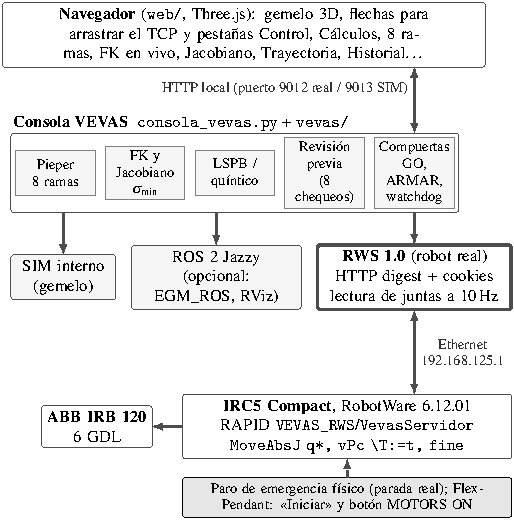
\includegraphics[width=\columnwidth]{fig_arquitectura.pdf}}
\caption{Arquitectura. Los modelos propios son comunes a los tres
backends; el paro de emergencia físico queda fuera de todo software.}
\label{fig:arq}
\end{figure}

Se eligió RWS porque solo exige PC Interface, no requiere instalar nada
en el controlador más allá de un módulo RAPID propio y no interfiere con
los módulos de otros grupos (\texttt{LabJointRws}, \texttt{EGM\_ROS},
\texttt{Imt342TrajectoryRapid}), que no se tocan. La compatibilidad con
RobotWare~6 impuso cuatro restricciones empíricas: \emph{(i)} al leer un
módulo por RWS su texto se trunca a 5000 caracteres, por lo que
\texttt{VEVAS\_RWS.mod} se mantiene bajo 4800 (hoy, 4123); \emph{(ii)}
los nombres globales deben ser únicos entre todos los módulos de
\texttt{T\_ROB1}, por lo que todo lo propio es \texttt{LOCAL} o lleva
prefijo \texttt{vv}; \emph{(iii)} el IRC5 admite pocas sesiones HTTP, y
al agotarlas responde 500 «Error registering callback», que se resuelve
cerrando sesión y reintentando; \emph{(iv)} tras un reinicio, «motores
ON» por RWS responde 403 y debe hacerlo el operador con el botón
MOTORS~ON. La autenticación es digest con la credencial de fábrica, que
no se publica.

\subsection{Modelos propios en vivo}

Los modelos de los Hitos~1 y~2 se ejecutan sin cambios sobre cada
muestra de juntas leída por RWS (10~Hz). La cinemática directa es
\begin{equation}
\begin{split}
  T_0^{\text{tool0}}(\bm q)&=\Big(\prod_{i=1}^{6}A_i(q_i)\Big)\,
     \mathrm{Rot}_z(\pi),\\
  A_i&=\mathrm{Rot}_z(\theta_i)\,\mathrm{Trans}_z(d_i)\,
      \mathrm{Trans}_x(a_i)\,\mathrm{Rot}_x(\alpha_i),
\end{split}
  \label{eq:fk}
\end{equation}
donde el giro final alinea el marco~6 de la tabla con el \texttt{tool0}
de ABB; con $\bm q=\bm 0$ la brida queda en $(0{,}374;\,0;\,0{,}630)$~m.

La inversa usa el desacople de Pieper \cite{b3}. Con
$\bm p_W=\bm p_6-d_6\bm z_6$, $L_3=\sqrt{a_3^2+d_4^2}$ y
$\gamma=\operatorname{atan2}(a_3,d_4)$:
\begin{equation}
\begin{split}
  q_1 &= \operatorname{atan2}(y_W,x_W)\ \ \text{o}\ \ +\pi,\qquad
  s=z_W-d_1,\\
  \cos\delta &= \frac{r^2+s^2-a_2^2-L_3^2}{2a_2L_3},\qquad
  q_3=\delta+\gamma-\tfrac{\pi}{2},\\
  q_2 &= \operatorname{atan2}(r,s)-
         \operatorname{atan2}(L_3\sin\delta,\ a_2+L_3\cos\delta),\\
  q_5 &= \operatorname{atan2}\!\big(\pm\sqrt{r_{13}^2+r_{23}^2},\ r_{33}\big),
  \quad R_3^6=(R_0^3)^{T}R_0^6,
\end{split}
\label{eq:pieper}
\end{equation}
con $r=\pm\sqrt{x_W^2+y_W^2}$; los tres signos binarios dan las ocho
ramas. Cada rama se reinyecta en \eqref{eq:fk} y se acepta si
$e_p<10^{-6}$~m y $e_R<10^{-5}$~rad.

Para la singularidad se escala la parte lineal del Jacobiano geométrico
con una longitud característica $L=0{,}3$~m \cite{b4}, de modo que filas lineales
y angulares sean comparables:
\begin{equation}
  J_L(\bm q)=\begin{bmatrix} I_3/L & 0\\ 0 & I_3\end{bmatrix}J(\bm q),
  \qquad \sigma_{\min}=\sigma_6(J_L).
  \label{eq:sigma}
\end{equation}
Un plan es \emph{singular} si $\sigma_{\min}<\sigma_u=0{,}02$ y está
«cerca» si $\sigma_{\min}<2\sigma_u$. El tipo se identifica con los
factores de la forma cerrada
$\det J=-a_2L_3\sin\delta\; r_W\sin q_5$: muñeca si $|\sin q_5|<0{,}09$,
codo si $|\sin\delta|<0{,}09$ y hombro si $r_W<0{,}03$~m.

\subsection{Protocolo PERS sobre RWS}

El módulo \texttt{VEVAS\_RWS} ejecuta la rutina \texttt{VevasServidor},
que al arrancar pide «Iniciar» en el FlexPendant
(\texttt{confirmarEnPendant}) y luego sondea cada 0{,}1~s. La
Fig.~\ref{fig:seq} resume un tramo. La PC escribe el objetivo articular
\texttt{vvPcTarget}, lo relee, comprueba que la postura medida no cambió
y recién entonces incrementa \texttt{vvPcSeq}; esa escritura es el
único acto que ordena movimiento. RAPID valida de nuevo y responde en
\texttt{vvRbCodigo}: 1 moviendo, 2 llegó, $-1$ vacío, $-2$ límites,
$-3$ paso $>45^\circ$, $-4$ modo no permitido. La PC solo da por
cumplido un tramo si \texttt{vvRbSeq} coincide, el código es~2 y la
postura \emph{medida} está a menos de $0{,}05^\circ$ del objetivo. Un
candado de archivo impide que dos herramientas escriban a la vez.

\begin{figure}[htbp]
\centerline{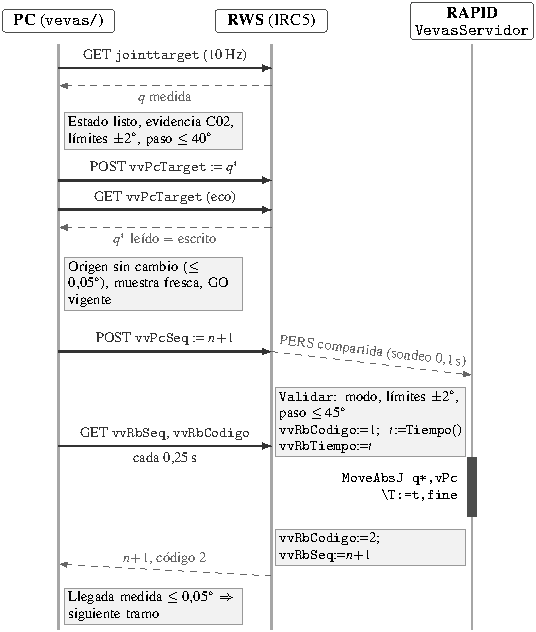
\includegraphics[width=0.97\columnwidth]{fig_secuencia.pdf}}
\caption{Secuencia de un tramo. Las validaciones de la PC (márgenes
$2^\circ$, paso $40^\circ$) son más estrictas que las de RAPID ($2^\circ$,
$45^\circ$), de modo que el controlador es la última barrera, no la
única.}
\label{fig:seq}
\end{figure}

\subsection{C02: velocidad por junta acotada en el controlador}
\label{sec:c02}

El requisito C02 exige que \emph{ninguna junta} supere su tope.
\texttt{MoveAbsJ} con \texttt{speeddata} solo limita la velocidad del
TCP y la reorientación, no cada eje. Por eso el RAPID calcula la
duración de cada tramo:
\begin{equation}
  t=\max\!\Big(0{,}5~\text{s},\ \max_i
     \frac{k_{\text{pico}}\,|\Delta q_i|}{v_{\lim,i}}\Big),
  \qquad k_{\text{pico}}=2{,}5,
  \label{eq:ley}
\end{equation}
con $v_{\lim}=[12{,}5;12{,}5;12{,}5;16;16;21]^\circ$/s, el 5\,\% de la
ficha (250/250/250/320/320/420~$^\circ$/s \cite{b5}), y mueve con
\texttt{MoveAbsJ q*, vPc \textbackslash T:=t, fine, tool0}. La PC no
puede pedir más velocidad: el tope vive en el controlador.

La justificación de $k_{\text{pico}}$ es la siguiente. Si el
controlador ejecuta el tramo con un perfil $q_i(\tau)=q_{i,0}+\Delta
q_i\,s(\tau/t)$, $s$ monótono de 0 a~1, la velocidad pico es
$c\,|\Delta q_i|/t$ con $c=\max s'$. Combinando con \eqref{eq:ley},
\begin{equation}
  \dot q_{i,\text{pico}}\le \frac{c}{k_{\text{pico}}}\,v_{\lim,i}.
  \label{eq:cota}
\end{equation}
Para perfiles usuales $c\le2$ (cúbico $1{,}5$, quíntico $1{,}875$,
trapezoidal entre 1 y 2, con 2 en el caso triangular), así que el pico
queda en $\le0{,}8\,v_{\lim,i}$: el factor 2{,}5 deja al menos un
20\,\% de margen frente a un perfil interno de ABB que no se conoce. Como $c$ no se conoce, se \emph{mide}
(Sec.~\ref{sec:res-c02}).

La herramienta \texttt{verificar\_c02.py} mueve cada junta $\pm\delta$
($\delta=5^\circ$ por defecto) y vuelve, muestrea \texttt{jointtarget}
de forma continua y estima la velocidad máxima por diferencias con
ventana de 0{,}10~s. La evidencia (\texttt{evidencia\_c02.json}) guarda
la huella SHA-256 del texto del módulo, el modo, $v_{\lim}$,
$k_{\text{pico}}$ y las seis juntas. El backend habilita el envío solo
si la evidencia pasó y su huella coincide con la del módulo local
\emph{y} con la del cargado en el IRC5, y si el modo actual es el
verificado: cambiar un carácter del \texttt{.mod} invalida la
autorización.

Cada trayectoria se muestrea y se parte en tramos \emph{colineales} en
el espacio articular de hasta $40^\circ$. Como \eqref{eq:ley} es lineal
en $|\Delta q|$ por encima del piso, partir un tramo en $n$ no cambia el
tiempo nominal total, pero agrega $n-1$ paradas en \texttt{fine}.

\subsection{Revisión previa y compuertas}

La Fig.~\ref{fig:tub} muestra el flujo de ocho pasos de la interfaz.
\texttt{revision.py} evalúa hasta 240 muestras del plan completo:
inicio en la postura medida ($\le1^\circ$), límites con margen
$\ge5^\circ$, velocidad del plan, $\sigma_{\min}$ y tipo de
singularidad, altura mínima del brazo (80~mm), autocolisión con
cápsulas \cite{b10}, entorno (mesa y cajas descritas) y herramienta. Cada chequeo
termina en \emph{aprobado}, \emph{aviso}, \emph{rechazado} o
\emph{no\_verificado}; con robot real, \emph{no\_verificado} bloquea,
porque «no se pudo evaluar» no equivale a «cumple». La
Tabla~\ref{tab:gates} lista las compuertas que se mantienen.

\begin{figure}[htbp]
\centerline{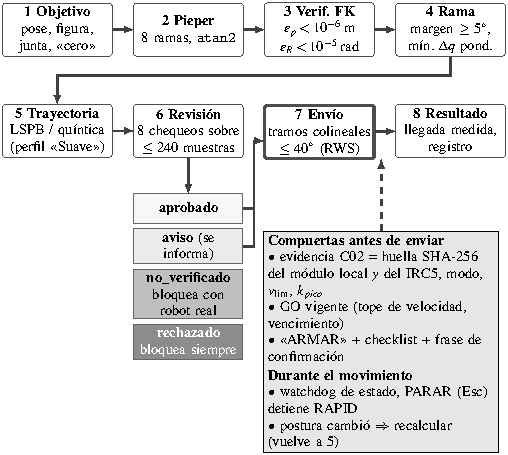
\includegraphics[width=\columnwidth]{fig_tuberia.pdf}}
\caption{Flujo de la interfaz, estados de la revisión y compuertas. Un
«aprobado» significa «cumple dentro del modelo», no «es seguro».}
\label{fig:tub}
\end{figure}

\begin{table}[htbp]
\caption{Compuertas de seguridad (software y física)}
\label{tab:gates}
\centering
\footnotesize
\begin{tabular}{@{}>{\raggedright}p{0.30\columnwidth}>{\raggedright\arraybackslash}p{0.64\columnwidth}@{}}
\toprule
\textbf{Compuerta} & \textbf{Qué impide} \\
\midrule
Revisión previa       & enviar un plan rechazado o no verificado \\
Evidencia C02         & mover con un módulo, topes o modo distintos de los medidos \\
GO (archivo JSON)     & mover sin autorización vigente; tope de velocidad y vencimiento \\
«ARMAR» + checklist   & enviar sin confirmación explícita y frase escrita \\
Validación RAPID      & límites $\pm2^\circ$, paso $>45^\circ$, modo no permitido \\
Watchdog de estado    & seguir con una muestra de juntas vieja \\
«Postura cambió»      & ejecutar un plan calculado desde otro origen \\
PARAR (Esc)           & detiene RAPID por RWS \\
Paro de emergencia    & parada física real; no depende de la PC \\
\bottomrule
\end{tabular}
\end{table}

Para la singularidad de muñeca se formalizaron dos excepciones, válidas
solo con RWS y C02 verificado, porque \texttt{MoveAbsJ} interpola en el
espacio articular y nunca invierte~$J$. Sea $\sigma_k$ la secuencia
muestreada, $\mathcal S=\{k:\sigma_k<\sigma_u\}$ y
$k^\ast=\arg\min_{k\in\mathcal S}\sigma_k$. \emph{Salir} de una
singularidad es aviso, y no rechazo, si
\begin{equation}
\begin{gathered}
 \mathcal S=\{0,\dots,m-1\},\ m<N,\quad
  \sigma_{k+1}\ge\sigma_k\ \ \forall\,k\in[k^\ast,m),\\
 \text{solo muñeca en }\mathcal S,\qquad \sigma_{N-1}\ge2\sigma_u ,
\end{gathered}
\label{eq:salida}
\end{equation}
es decir, la zona singular es un tramo inicial contiguo y el camino se
aleja monótonamente desde el mínimo. La condición sobre $k^\ast$ admite
que el robot arranque con $q_5$ apenas del otro lado de cero
($-0{,}05^\circ$ leídos por RWS) y cruce el mínimo. La excepción
simétrica, \emph{llegar} a $\bm q=\bm 0$, exige un tramo singular
contiguo que termina en la última muestra con $\sigma$ no creciente.
Entrar a una singularidad en cualquier otro caso sigue siendo
\emph{rechazado}.

% =====================================================================
\section{Resultados}
\label{sec:res}

\subsection{Modelos propios contra el controlador}

La validación fuera de línea (bitácora S0-001) dio error de FK de
$6\times10^{-16}$~m en 5000 posturas, Jacobiano contra diferencias
finitas de $9\times10^{-11}$~m/rad y una amplificación
$\lVert\dot{\bm q}\rVert\sim q_5^{-1{,}00}$, coherente con el Hito~2.
Dos casos de control negativo ---TCP desplazado y orden de factores
alterado--- fallan a propósito con $0{,}120$~m y $0{,}469$~rad: la
prueba es sensible a los errores que dice detectar.

En presencia del robot (24/11), las seis juntas leídas por RWS
coincidieron con el FlexPendant, y la FK propia con \texttt{tool0},
\texttt{wobj0} y base difirió de la del controlador en 0{,}0001~mm y
0{,}0000$^\circ$. Tras actualizar los contadores de revoluciones
(Sec.~\ref{sec:inc}) el diagnóstico volvió a dar 0{,}0000~mm con las
juntas cerca de cero. La suite automática suma 265 pruebas en Python
(pytest, incluido un IRC5 simulado por HTTP con un perfil que
\emph{no} respeta el tiempo, para comprobar que la evidencia falla) y 10
en JavaScript, todas aprobadas.

\subsection{Velocidad articular medida (C02)}
\label{sec:res-c02}

La Tabla~\ref{tab:c02} y la Fig.~\ref{fig:c02} resumen la verificación
presencial en AUTO. Con $\delta=5^\circ$, \eqref{eq:ley} da
$t=2{,}5\cdot5/12{,}5=1{,}00$~s en J1--J3, 0{,}78~s en J4--J5 y 0{,}60~s
en J6; la herramienta exige además que \texttt{vvRbTiempo} coincida con
el valor esperado. Las
velocidades medias nominales $\delta/t=v_{\lim}/k_{\text{pico}}$ son
5{,}0, 6{,}4 y 8{,}4~$^\circ$/s; las máximas medidas, 5{,}2--8{,}9.

\begin{table}[htbp]
\caption{Verificación C02 en el IRB~120 real (AUTO, 24/11/2026)}
\label{tab:c02}
\centering
\footnotesize
\begin{tabular}{@{}lccccc@{}}
\toprule
\textbf{Juntas} & $v_{\lim}$ & $t$ [s] & $\delta/t$ & $v_{\max}$ medida & $v_{\max}/v_{\lim}$ \\
 & [$^\circ$/s] & & [$^\circ$/s] & [$^\circ$/s] & \\
\midrule
J1--J3 & 12.5 & 1.00 & 5.0 & 5.2--5.4 & 0.42--0.43 \\
J4--J5 & 16   & 0.78 & 6.4 & 6.7--6.9 & 0.42--0.43 \\
J6     & 21   & 0.60 & 8.4 & 8.8--8.9 & 0.42 \\
\bottomrule
\end{tabular}
\end{table}

\begin{figure}[htbp]
\centerline{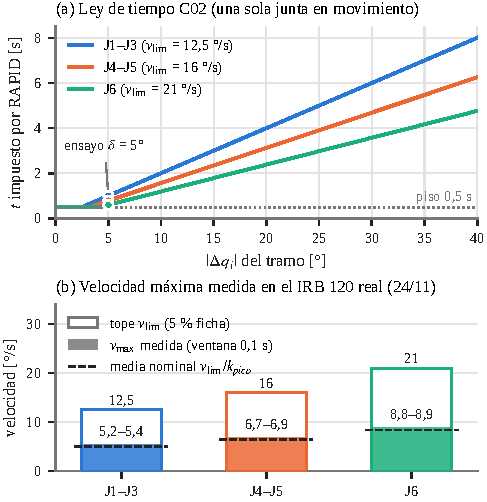
\includegraphics[width=\columnwidth]{fig_c02.pdf}}
\caption{(a) Duración impuesta por \eqref{eq:ley} según la junta que
domina; los puntos marcan el ensayo. (b) Velocidad máxima medida frente
al tope y a la media nominal.}
\label{fig:c02}
\end{figure}

El cociente pico/medio medido es $\approx1{,}06$, muy por debajo de la
cota $c\le2$ supuesta en \eqref{eq:cota}: el perfil que genera el IRC5 para
\texttt{MoveAbsJ \textbackslash T} en tramos cortos es casi de velocidad
constante, y el pico real queda en el 42--43\,\% de $v_{\lim}$, es decir,
$\approx2{,}2$\,\% de la ficha. Todas las juntas pasaron.

\subsection{La postura de reposo es singular}

$\sigma_{\min}(\bm 0)=1{,}2\times10^{-16}$: con $q_5=0$ los ejes 4 y 6
se alinean. La Fig.~\ref{fig:sigma} muestra $\sigma_{\min}$, calculado
con los módulos del proyecto, sobre los dos movimientos que conectan el
trabajo con esa postura. «Volver a cero» desde la postura inicial
$[0,-20,30,0,40,0]^\circ$ parte de $\sigma=0{,}261$ y llega a cero; con
RWS y C02 la revisión lo da como \emph{aviso} y el mismo plan sin la
excepción es \emph{rechazado}. «Preparar J5 a $+30^\circ$» sube
monótonamente hasta $0{,}231$ y cumple \eqref{eq:salida}. Ambos caben en
un solo tramo; \eqref{eq:ley} les asigna 6{,}25~s (domina J5 con
$40^\circ$) y 4{,}69~s.

\begin{figure}[htbp]
\centerline{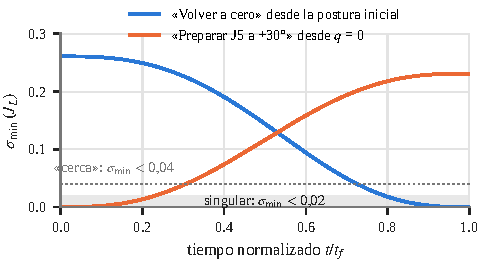
\includegraphics[width=\columnwidth]{fig_sigma.pdf}}
\caption{$\sigma_{\min}(J_L)$ a lo largo de los dos movimientos que
tocan $\bm q=\bm 0$. Gris: zona singular ($\sigma_u=0{,}02$).}
\label{fig:sigma}
\end{figure}

\subsection{Figuras sobre el robot real}

Las figuras predeterminadas (círculo, corazón, cuadrado, triángulo y un
saludo articular de muñeca) se resuelven con Pieper punto a punto, con
orientación constante, salto articular máximo de $12^\circ$ entre
puntos y paradas en esquinas y cúspides. En el robot real se limitan a
80~mm y exigen RWS con C02. Pasar los tramos de $10^\circ$ a $40^\circ$
eliminó las pausas visibles en los recorridos largos: para «Volver a
cero», 4 paradas en \texttt{fine} se reducen a una, con el mismo
tiempo nominal de 6{,}25~s.

% =====================================================================
\section{Discusión y análisis de fallas}
\label{sec:inc}

\subsection{Dónde vive el tope importa}

Un tope impuesto en la PC depende de que la PC funcione bien; uno
impuesto en RAPID, no. Por eso \eqref{eq:ley} se calcula en el
controlador y la PC solo la \emph{replica} para estimar duraciones. La
medición confirma la cota \eqref{eq:cota} con amplio margen, pero lo
relevante es que la evidencia acredita una combinación concreta de
módulo, topes y modo. Una verificación en AUTO no autoriza manual, y un
módulo editado exige medir de nuevo.

\subsection{Singularidad: aviso no es permiso}

El Hito~2 mostró que el LSPB atraviesa $q_5=0$ sin dificultad porque
interpola en el espacio articular. Aquí esa observación se vuelve
regla: con \texttt{MoveAbsJ} y velocidad por junta acotada, llegar a
$\bm q=\bm 0$ o salir de ella no produce velocidades explosivas, de modo
que bloquearlas dejaría al robot sin salida desde su propio reposo. Pero
la excepción es estrecha ---solo muñeca, monótona, contigua--- y
el aviso recuerda que desde ahí no se debe mover en cartesiano.

\subsection{Incidentes analizados}

La Tabla~\ref{tab:inc} resume las cinco fallas de campo; las dos
últimas fueron defectos propios.

\begin{table}[htbp]
\caption{Incidentes de laboratorio (bitácora) y acción tomada}
\label{tab:inc}
\centering
\footnotesize
\setlength{\tabcolsep}{3pt}
\begin{tabular}{@{}>{\raggedright}p{0.03\columnwidth}>{\raggedright}p{0.42\columnwidth}>{\raggedright\arraybackslash}p{0.50\columnwidth}@{}}
\toprule
\# & \textbf{Síntoma / causa} & \textbf{Acción y aprendizaje} \\
\midrule
1 & RAPID de otro grupo corriendo & el script no arranca encima; se pidió detenerlo \\
2 & RWS sin respuesta (HTTP 000, ping OK) & reinicio; antes, STOP (evento 20054), luego paro, rearme y MOTORS ON \\
3 & Contadores de revoluciones perdidos (20082), batería SMB débil & ejes a marcas de sincronización, contadores actualizados, FK = 0{,}0000~mm; cambiar batería \\
4 & Bug propio: instalar el módulo apagaba motores encendidos & solo se apagan si hay que escribir; ante 403 se espera 60~s al operador \\
5 & Pausas: tramos de $10^\circ$ con \texttt{fine} & tramos colineales de $40^\circ$ \\
\bottomrule
\end{tabular}
\end{table}

El incidente~3 es el más instructivo. Tras perder la referencia de las
vueltas de motor, el robot puede \emph{creer} estar en una postura y
estar en otra; ningún modelo cinemático, por exacto que sea, lo detecta,
porque compara contra las mismas lecturas. La única verificación válida
fue física: llevar los ejes a las marcas y recién entonces volver a
comparar FK. El incidente~4 muestra un efecto de segundo orden de una
medida de seguridad: apagar motores «por las dudas» dejó al sistema en
un estado del que la PC no podía salir sola.

% =====================================================================
\section{Limitaciones y trabajo futuro}

\emph{Paradas entre puntos.} Cada tramo termina en \texttt{fine}, de
modo que las figuras de muchos puntos se detienen en cada vértice no
colineal. Está en desarrollo, todavía sin publicar, un modo de
\emph{streaming} con zonas \texttt{z1}: variable \texttt{vvPcZona}, piso
$t_{\text{zona}}=0{,}2$~s y $\Delta q$ medido contra el objetivo previo
en lugar de la postura actual. Al cambiar el módulo, exigirá repetir
\texttt{verificar\_c02}.

\emph{Medición.} La velocidad se estima por diferencias de posiciones
leídas por RWS con ventana de 0{,}1~s, no con una traza interna del
controlador: el promedio en la ventana puede subestimar un pico breve.
El margen de \eqref{eq:cota} cubre ese sesgo, pero no lo elimina.

\emph{Modelo de entorno.} La revisión ve solo lo descrito: cápsulas que
aproximan los eslabones, la mesa y las cajas declaradas, y evalúa a lo
sumo 240 muestras; entre ellas no se garantiza nada. La FK en vivo se
comparó en pocas posturas.

\emph{Hardware.} La batería SMB debe reemplazarse y conviene verificar la
calibración fina desde el FlexPendant.

Como trabajo futuro quedan una cámara cenital con calibración DLT propia
(error $<1{,}5$~mm), una pinza neumática por E/S y EGM para control
articular a 250~Hz.

% =====================================================================
\section{Conclusiones}

Los modelos propios de los Hitos~1 y~2 comandan hoy al IRB~120 real sin
modificaciones: la FK coincide con la del controlador a 0{,}0001~mm, y
Pieper, el Jacobiano y $\sigma_{\min}$ operan en vivo sobre cada lectura.
El aporte de ingeniería de este hito no fue un modelo nuevo sino la
capa que hace confiable el envío: un protocolo con doble validación y
acuse medido, una ley de tiempo impuesta en el controlador y una
evidencia medida que solo vale para el módulo que la produjo. Las
velocidades medidas quedaron en el 42--43\,\% del tope.

Dos lecciones exceden al proyecto. La primera: la postura de reposo de
fábrica es singular, y tratarlo bien exige criterios sobre el
\emph{camino}, no sobre puntos aislados. La segunda: las fallas más
peligrosas observadas ---contadores perdidos, motores apagados sin
necesidad--- no eran errores de cálculo, sino de estado; por eso el paro
de emergencia y el operador siguen siendo la última compuerta.

\begin{thebibliography}{00}
\bibitem{b1} B. Siciliano, L. Sciavicco, L. Villani y G. Oriolo,
\textit{Robotics: Modelling, Planning and Control}. Springer, 2009.
\bibitem{b2} J. J. Craig, \textit{Introduction to Robotics: Mechanics
and Control}, 4.ª ed. Pearson, 2018.
\bibitem{b3} D. L. Pieper, ``The kinematics of manipulators under
computer control,'' tesis doctoral, Univ.\ de Stanford, 1968.
\bibitem{b4} T. Yoshikawa, ``Manipulability of robotic mechanisms,''
\textit{Int.\ J. Robot.\ Res.}, vol.~4, n.º~2, pp.~3--9, 1985.
\bibitem{b5} ABB Robotics, \textit{Product Specification IRB 120},
doc.\ 3HAC035960-001, 2023.
\bibitem{b6} ABB Robotics, \textit{Robot Web Services (RWS 1.0) para
RobotWare~6} y \textit{Technical Reference Manual: RAPID Instructions,
Functions and Data Types}. ABB, documentación de RobotWare~6.
\bibitem{b7} Grupo VEVAS, ``Gemelo digital cinemático del manipulador
ABB IRB 120,'' informe del Hito~1, IMT-342, UCB Tarija, 2026.
\bibitem{b8} Grupo VEVAS, ``Integración de modelos cinemáticos,
diferenciales y dinámicos para manipuladores: validación sobre el ABB
IRB~120,'' informe del Hito~2, IMT-342, UCB Tarija, 2026.
\bibitem{b9} Grupo VEVAS, ``PFI --- ABB IRB 120,'' repositorio, 2026.
[En línea]. \url{https://github.com/FlorenciaFrigerio/pfi-vevas-irb120}
\bibitem{b10} C. Ericson, \textit{Real-Time Collision Detection}. Morgan
Kaufmann, 2005.
\bibitem{b11} B. Quiroga Turdera, ``Guía y rúbrica: ECI-3/4,''
IMT-342, Universidad Católica Boliviana ``San Pablo'', 2026.
\end{thebibliography}

\end{document}
